% Diagram: RNN Sequential Processing
\begin{figure}[htbp]
\centering
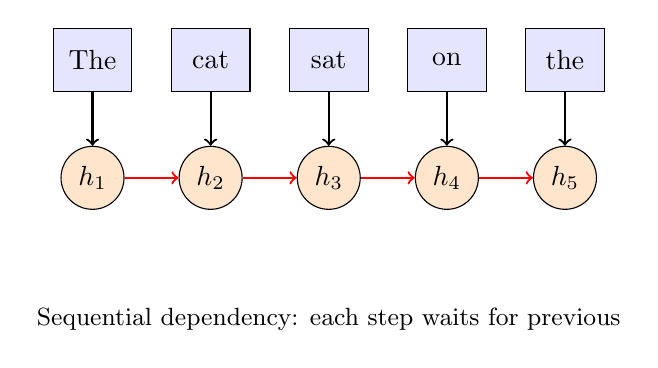
\begin{tikzpicture}[
    node distance=1.5cm,
    token/.style={rectangle, draw, minimum width=1cm, minimum height=0.8cm, fill=blue!10},
    hidden/.style={circle, draw, minimum size=0.8cm, fill=orange!20},
    arrow/.style={->, thick}
]
% Tokens
\node[token] (t1) {The};
\node[token, right of=t1] (t2) {cat};
\node[token, right of=t2] (t3) {sat};
\node[token, right of=t3] (t4) {on};
\node[token, right of=t4] (t5) {the};

% Hidden states
\node[hidden, below of=t1] (h1) {$h_1$};
\node[hidden, below of=t2] (h2) {$h_2$};
\node[hidden, below of=t3] (h3) {$h_3$};
\node[hidden, below of=t4] (h4) {$h_4$};
\node[hidden, below of=t5] (h5) {$h_5$};

% Vertical arrows (token to hidden)
\draw[arrow] (t1) -- (h1);
\draw[arrow] (t2) -- (h2);
\draw[arrow] (t3) -- (h3);
\draw[arrow] (t4) -- (h4);
\draw[arrow] (t5) -- (h5);

% Horizontal arrows (sequential dependency)
\draw[arrow, red, thick] (h1) -- (h2);
\draw[arrow, red, thick] (h2) -- (h3);
\draw[arrow, red, thick] (h3) -- (h4);
\draw[arrow, red, thick] (h4) -- (h5);

% Labels
\node[below of=h3, yshift=-0.3cm] {\small Sequential dependency: each step waits for previous};
\end{tikzpicture}
\caption{RNN processing: each hidden state depends on the previous, forcing sequential execution.}
\label{fig:rnn-sequential}
\end{figure}
